\documentclass[11pt]{article}

\usepackage[T1]{fontenc}
\usepackage[margin=1in]{geometry}
\usepackage{amsmath}
\usepackage{float}
\usepackage{xcolor}
\usepackage{listings}
\usepackage{algorithm}
\usepackage{algpseudocode}
\usepackage{booktabs}
\usepackage{tikz}
\usepackage{graphicx}

\definecolor{shellbg}{HTML}{F5F5F5}
\definecolor{rulegray}{HTML}{BBBBBB}
\definecolor{commentgray}{HTML}{6A737D}

\lstdefinestyle{term}{
  basicstyle=\ttfamily\scriptsize,
  backgroundcolor=\color{shellbg},
  frame=single, rulecolor=\color{rulegray},
  breaklines=true, columns=fullflexible, keepspaces=true,
  showstringspaces=false, xleftmargin=6pt, xrightmargin=6pt,
  aboveskip=6pt, belowskip=6pt,
}
\lstdefinestyle{code}{
  language=C++,
  basicstyle=\ttfamily\scriptsize,
  keywordstyle=\bfseries,
  commentstyle=\color{commentgray}\itshape,
  numbers=left, numberstyle=\tiny\color{commentgray}, numbersep=6pt,
  frame=single, rulecolor=\color{rulegray},
  breaklines=true, columns=fullflexible, keepspaces=true,
  showstringspaces=false, xleftmargin=16pt, xrightmargin=6pt,
  aboveskip=6pt, belowskip=6pt,
}

\algrenewcommand\algorithmicrequire{\textbf{Input:}}
\algrenewcommand\algorithmicensure{\textbf{Output:}}

\setlength{\parindent}{0pt}
\setlength{\parskip}{0.42em plus 0.1em minus 0.12em}
\setlength{\textfloatsep}{8pt plus 2pt minus 2pt}
\setlength{\intextsep}{8pt plus 2pt minus 2pt}

\begin{document}

\section*{Problem 1: Bubble Sort}

\textbf{Approach.} Compare neighbouring elements and swap them if they are out of order. Each pass
moves the largest unsorted value to the end. If a pass makes no swap, the array is sorted and the
loop stops.

\begin{algorithm}[H]
\caption{Bubble Sort}
\begin{algorithmic}[1]
\Require An array $A$ of $n$ numbers
\Ensure $A$ sorted in increasing order
\For{$last \gets n-1$ \textbf{downto} $1$}
    \State $swapped \gets \textbf{false}$
    \For{$j \gets 0$ \textbf{to} $last-1$}
        \If{$A[j] > A[j+1]$}
            \State \Call{Swap}{$A[j], A[j+1]$}
            \State $swapped \gets \textbf{true}$
        \EndIf
    \EndFor
    \State \Call{PrintArray}{$A, n$}
    \If{$swapped = \textbf{false}$}
        \State \textbf{break}
    \EndIf
\EndFor
\end{algorithmic}
\end{algorithm}

\textbf{C++ code.}
\lstinputlisting[style=code]{cpp/Assignment01_Problem01_Suh.cpp}

\noindent\begin{minipage}{\linewidth}
\textbf{Output.}\\[4pt]
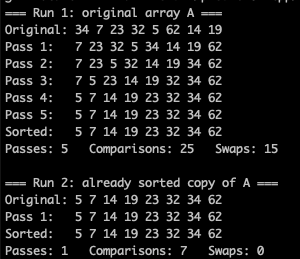
\includegraphics[width=0.33\linewidth]{screenshots/problem01.png}
\end{minipage}

\textbf{Item 5.} On the sorted copy: 1 pass, 7 comparisons, 0 swaps. No pair is out of order, so the
first pass makes no swap, $swapped$ stays false, and the loop stops.

\newpage

\section*{Problem 2: Insertion Sort}

\textbf{Approach.} Take each element as the key, shift the larger elements of the sorted part one
position right, and insert the key into the gap.

\begin{algorithm}[H]
\caption{Insertion Sort}
\begin{algorithmic}[1]
\Require An array $A$ of $n$ numbers
\Ensure $A$ sorted in increasing order
\For{$i \gets 1$ \textbf{to} $n-1$}
    \State $key \gets A[i]$
    \State $j \gets i-1$
    \While{$j \ge 0$ \textbf{and} $A[j] > key$}
        \State $A[j+1] \gets A[j]$
        \State $j \gets j-1$
    \EndWhile
    \State $A[j+1] \gets key$
    \State Print $i$, $key$ and \Call{PrintArray}{$A, n$}
\EndFor
\end{algorithmic}
\end{algorithm}

\textbf{C++ code.}
\lstinputlisting[style=code]{cpp/Assignment01_Problem02_Suh.cpp}

\noindent\begin{minipage}{\linewidth}
\textbf{Output.}\\[4pt]
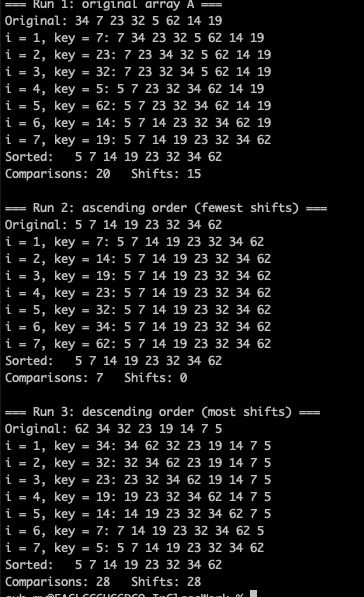
\includegraphics[width=0.40\linewidth]{screenshots/problem02.png}
\end{minipage}

\textbf{Item 4.} Fewest shifts: ascending order 5 7 14 19 23 32 34 62 (0 shifts). Most shifts:
descending order 62 34 32 23 19 14 7 5 (28 shifts). Each shift fixes one pair that is out of order;
ascending order has no such pair and descending order has all $n(n-1)/2 = 28$ of them.

\newpage

\section*{Problem 3: Selection Sort}

\textbf{Approach.} In each pass, find the smallest value in the unsorted part and swap it into the
first unsorted position. Skip the swap if it is already there.

\begin{algorithm}[H]
\caption{Selection Sort}
\begin{algorithmic}[1]
\Require An array $A$ of $n$ numbers
\Ensure $A$ sorted in increasing order
\For{$i \gets 0$ \textbf{to} $n-2$}
    \State $minIdx \gets i$
    \For{$j \gets i+1$ \textbf{to} $n-1$}
        \If{$A[j] < A[minIdx]$}
            \State $minIdx \gets j$
        \EndIf
    \EndFor
    \If{$minIdx \ne i$}
        \State \Call{Swap}{$A[i], A[minIdx]$}
    \EndIf
    \State Print $A[i]$, $minIdx$ and \Call{PrintArray}{$A, n$}
\EndFor
\end{algorithmic}
\end{algorithm}

\textbf{C++ code.}
\lstinputlisting[style=code]{cpp/Assignment01_Problem03_Suh.cpp}

\noindent\begin{minipage}{\linewidth}
\textbf{Output.}\\[4pt]
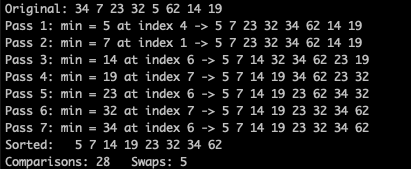
\includegraphics[width=0.45\linewidth]{screenshots/problem03.png}
\end{minipage}

\textbf{Item 4.} Selection Sort makes 5 swaps on $A$ and Bubble Sort makes 15. Selection Sort makes
at most one swap per pass, because it finds the minimum first and moves it directly to its final
position. Bubble Sort only swaps neighbours, and each swap fixes only one pair that is out of order,
so it needs one swap for each of the 15 such pairs in $A$.

\newpage

\section*{Problem 4: Quick Sort}

\textbf{Approach.} Use the last element as the pivot. The partition moves the smaller values to the
left of the pivot and puts the pivot in its final position. Then sort the left and right parts
recursively.

\begin{algorithm}[H]
\caption{Quick Sort (Lomuto partition)}
\begin{algorithmic}[1]
\Require An array $A$ and indices $low$, $high$
\Ensure $A[low..high]$ sorted in increasing order
\Procedure{QuickSort}{$A, low, high, depth$}
    \If{$low < high$}
        \State Print $depth$ indentation, $A[high]$ and \Call{PrintArray}{$A[low..high]$}
        \State $p \gets \Call{Partition}{A, low, high}$
        \State \Call{QuickSort}{$A, low, p-1, depth+1$}
        \State \Call{QuickSort}{$A, p+1, high, depth+1$}
    \EndIf
\EndProcedure
\Procedure{Partition}{$A, low, high$}
    \State $pivot \gets A[high]$
    \State $i \gets low - 1$
    \For{$j \gets low$ \textbf{to} $high-1$}
        \If{$A[j] < pivot$}
            \State $i \gets i + 1$
            \State \Call{Swap}{$A[i], A[j]$}
            \State Print $i$, $j$ and \Call{PrintArray}{$A[low..high]$} (first partition only)
        \EndIf
    \EndFor
    \State \Call{Swap}{$A[i+1], A[high]$}
    \State Print the pivot position $i+1$ (first partition only)
    \State \Return $i+1$
\EndProcedure
\end{algorithmic}
\end{algorithm}

\textbf{C++ code.}
\lstinputlisting[style=code]{cpp/Assignment01_Problem04_Suh.cpp}

\noindent\begin{minipage}{\linewidth}
\textbf{Output.}\\[4pt]
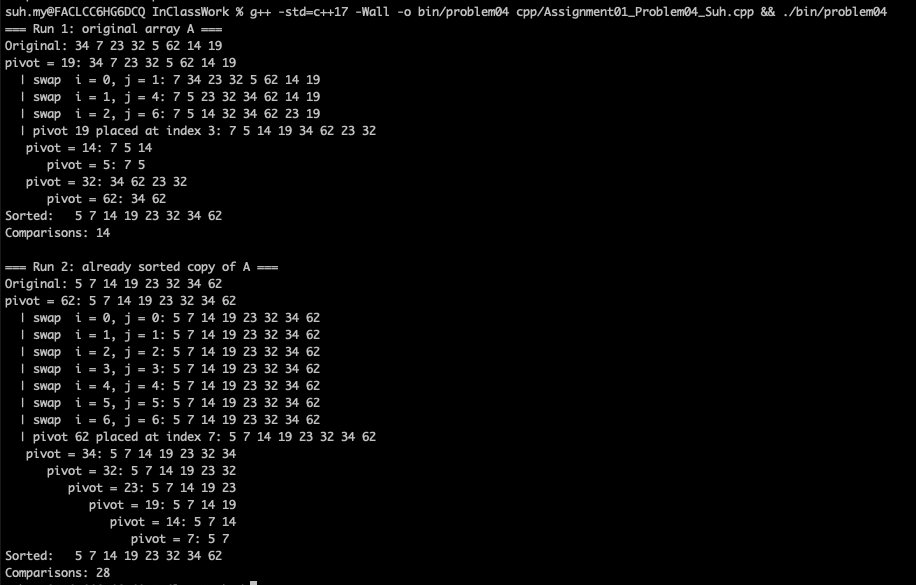
\includegraphics[width=1.00\linewidth]{screenshots/problem04.png}
\end{minipage}

\textbf{Item 5.} On the sorted copy Quick Sort makes 28 comparisons instead of 14. In a sorted array
the last element is always the largest, so each partition leaves all the other elements on one side
and the problem shrinks by only one element per call: $7 + 6 + \dots + 1 = n(n-1)/2 = 28$
comparisons, $O(n^2)$. To avoid it, choose the pivot at random or use the median of the first,
middle and last elements.

\newpage

\section*{Problem 5: Merge Sort}

\textbf{Approach.} Split the array at $mid = (low + high)/2$, sort each half recursively, and merge
the two sorted halves by repeatedly taking the smaller front element.

\begin{algorithm}[H]
\caption{Merge Sort}
\begin{algorithmic}[1]
\Require An array $A$ and indices $low$, $high$
\Ensure $A[low..high]$ sorted in increasing order
\Procedure{MergeSort}{$A, low, high$}
    \If{$low < high$}
        \State Print ``split:'' and \Call{PrintArray}{$A[low..high]$}
        \State $mid \gets \lfloor (low + high)/2 \rfloor$
        \State \Call{MergeSort}{$A, low, mid$}
        \State \Call{MergeSort}{$A, mid+1, high$}
        \State \Call{Merge}{$A, low, mid, high$}
        \State Print ``merged:'' and \Call{PrintArray}{$A[low..high]$}
    \EndIf
\EndProcedure
\Procedure{Merge}{$A, low, mid, high$}
    \State $L \gets A[low..mid]$;\quad $R \gets A[mid+1..high]$
    \State $i \gets 0$;\quad $j \gets 0$;\quad $k \gets low$
    \While{$i < |L|$ \textbf{and} $j < |R|$}
        \If{$L[i] \le R[j]$}
            \State $A[k] \gets L[i]$;\quad $i \gets i+1$
        \Else
            \State $A[k] \gets R[j]$;\quad $j \gets j+1$
        \EndIf
        \State $k \gets k+1$
    \EndWhile
    \State Copy the rest of $L$ and $R$ into $A[k..high]$
\EndProcedure
\end{algorithmic}
\end{algorithm}

\textbf{C++ code.}
\lstinputlisting[style=code]{cpp/Assignment01_Problem05_Suh.cpp}

\noindent\begin{minipage}{\linewidth}
\textbf{Output.}\\[4pt]
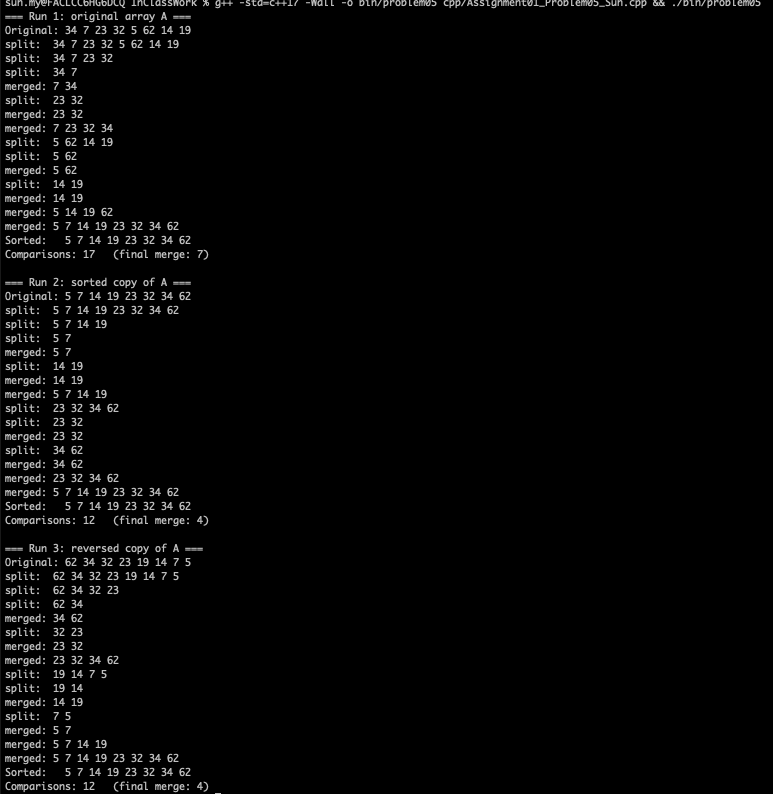
\includegraphics[width=0.84\linewidth]{screenshots/problem05.png}
\end{minipage}

\textbf{Item 5.} Comparisons: 17 for $A$, 12 for the sorted copy, 12 for the reversed copy. The
splits depend only on $n$, so the same merges happen for every order; the order only changes how
early each merge runs out of one half. Bubble Sort (7 to 28) and Quick Sort (14 to 28) change much
more because their work depends on the order. Merge Sort needs $O(n)$ extra memory for the
temporary arrays used in merging.

\newpage

\section*{Problem 6: Heap Sort}

\textbf{Approach.} Build a max-heap, where every parent is at least as large as its children. Then
repeatedly swap the root (the maximum) with the last element of the heap, shrink the heap by one,
and sift the new root down.

\begin{algorithm}[H]
\caption{Heap Sort}
\begin{algorithmic}[1]
\Require An array $A$ of $n$ numbers
\Ensure $A$ sorted in increasing order
\Procedure{SiftDown}{$A, root, size$}
    \Loop
        \State $largest \gets root$;\quad $left \gets 2 \cdot root + 1$;\quad $right \gets 2 \cdot root + 2$
        \If{$left < size$ \textbf{and} $A[left] > A[largest]$}
            \State $largest \gets left$
        \EndIf
        \If{$right < size$ \textbf{and} $A[right] > A[largest]$}
            \State $largest \gets right$
        \EndIf
        \If{$largest = root$}
            \State \Return
        \EndIf
        \State \Call{Swap}{$A[root], A[largest]$}
        \State $root \gets largest$
    \EndLoop
\EndProcedure
\Procedure{HeapSort}{$A, n$}
    \For{$root \gets \lfloor n/2 \rfloor - 1$ \textbf{downto} $0$}
        \State \Call{SiftDown}{$A, root, n$}
    \EndFor
    \State Print ``Heap:'' and \Call{PrintArray}{$A, n$}
    \For{$end \gets n-1$ \textbf{downto} $1$}
        \State \Call{Swap}{$A[0], A[end]$}
        \State \Call{SiftDown}{$A, 0, end$}
        \State \Call{PrintArray}{$A[0..end-1]$};\quad \Call{PrintArray}{$A[end..n-1]$}
    \EndFor
\EndProcedure
\end{algorithmic}
\end{algorithm}

\textbf{Heap after building:} 62 32 34 19 5 23 14 7

\begin{center}
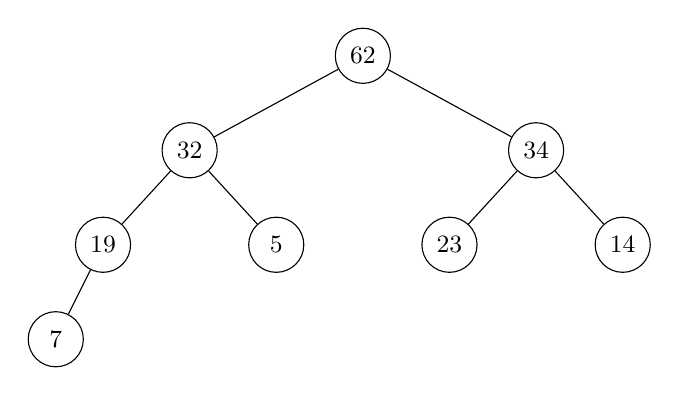
\begin{tikzpicture}[
  every node/.style={circle, draw, minimum size=7mm, inner sep=0pt, font=\small},
  level 1/.style={sibling distance=44mm},
  level 2/.style={sibling distance=22mm},
  level 3/.style={sibling distance=12mm},
  level distance=12mm]
\node {62}
  child {node {32}
    child {node {19}
      child {node {7}}
      child[missing]}
    child {node {5}}}
  child {node {34}
    child {node {23}}
    child {node {14}}};
\end{tikzpicture}
\end{center}

\textbf{C++ code.}
\lstinputlisting[style=code]{cpp/Assignment01_Problem06_Suh.cpp}

\noindent\begin{minipage}{\linewidth}
\textbf{Output.}\\[4pt]
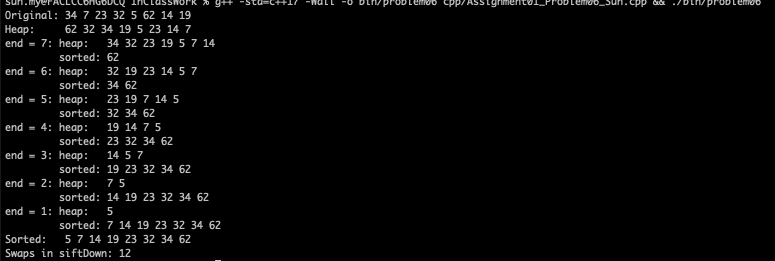
\includegraphics[width=0.85\linewidth]{screenshots/problem06.png}
\end{minipage}

\textbf{Item 5.} Heap Sort is not stable. Example: $[4_a, 4_b, 1]$, which is already a max-heap.
Swapping the root to the end gives $[1, 4_b, 4_a]$, sifting down gives $[4_b, 1, 4_a]$, and the last
swap gives $[1, 4_b, 4_a]$. The two equal values end up in reverse order.

\newpage

\section*{Problem 7: Comparing the Six Algorithms}

\textbf{Approach.} The program uses the six sorts from Problems 1--6 without printing, and each one
counts its comparisons. For timing, every algorithm sorts a fresh copy of the same random data
(values 1--100{,}000, fixed seed), and the time is the average of 5 runs.

\begin{algorithm}[H]
\caption{Comparing the algorithms}
\begin{algorithmic}[1]
\For{each input $X \in \{A, \text{sorted } A, \text{reversed } A\}$}
    \For{each algorithm \textsc{Sort}}
        \State Sort a copy of $X$ and record the comparisons
    \EndFor
\EndFor
\For{each $n \in \{1000, 5000, 10000\}$}
    \State $data \gets n$ random values in $[1, 100000]$
    \For{each algorithm \textsc{Sort}}
        \State Time \textsc{Sort} on a fresh copy of $data$ 5 times and take the average
        \State \Call{PrintArray}{$work, 10$}
    \EndFor
\EndFor
\end{algorithmic}
\end{algorithm}

\textbf{Item 1: comparisons.}

\begin{center}
\small
\begin{tabular}{@{}lccc@{}}
\toprule
Algorithm & $A$ & Sorted & Reversed \\
\midrule
Bubble Sort & 25 & 7 & 28 \\
Insertion Sort & 20 & 7 & 28 \\
Selection Sort & 28 & 28 & 28 \\
Quick Sort & 14 & 28 & 28 \\
Merge Sort & 17 & 12 & 12 \\
Heap Sort & 26 & 27 & 24 \\
\bottomrule
\end{tabular}
\end{center}

\textbf{Item 2: running time (ms).}

\begin{center}
\small
\begin{tabular}{@{}lrrrr@{}}
\toprule
Algorithm & $n = 1{,}000$ & $n = 5{,}000$ & $n = 10{,}000$ & $10{,}000 / 1{,}000$ \\
\midrule
Bubble Sort & 0.276 & 5.831 & 22.107 & 80.1 \\
Insertion Sort & 0.077 & 1.472 & 5.685 & 73.8 \\
Selection Sort & 0.789 & 19.229 & 73.981 & 93.7 \\
Quick Sort & 0.015 & 0.124 & 0.442 & 29.0 \\
Merge Sort & 0.059 & 0.232 & 0.750 & 12.6 \\
Heap Sort & 0.023 & 0.147 & 0.591 & 26.0 \\
\bottomrule
\end{tabular}
\end{center}

\textbf{C++ code.}
\lstinputlisting[style=code]{cpp/Assignment01_Problem07_Suh.cpp}

\noindent\begin{minipage}{\linewidth}
\textbf{Output.}\\[4pt]
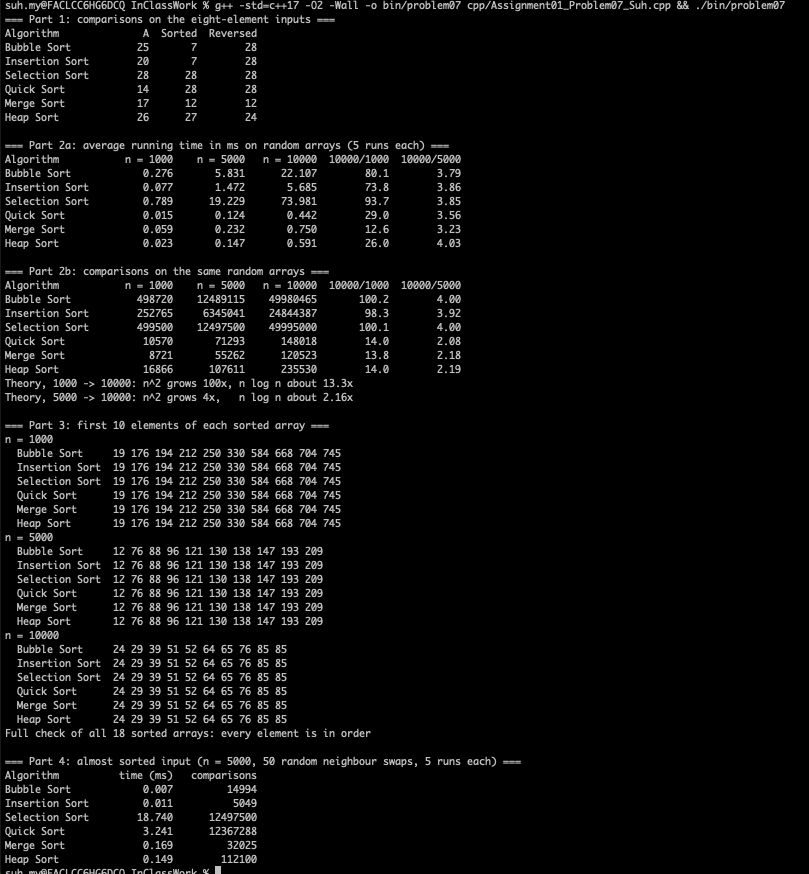
\includegraphics[width=0.88\linewidth]{screenshots/problem07.png}
\end{minipage}

\textbf{Item 4.}
\begin{itemize}
\item Bubble, Insertion and Selection Sort grow like $n^2$. Quick, Merge and Heap Sort grow like
$n \log n$.
\item Mostly. From 1{,}000 to 10{,}000 values the $n^2$ sorts took 74 to 94 times longer
(theory: 100) and the $n \log n$ sorts 13 to 29 times longer (theory: 13.3). The $n \log n$ times
are under 1 ms, so they are noisier, but the comparison counts grow almost exactly as predicted:
about 100 times for the $n^2$ sorts and 14 times for the $n \log n$ sorts.
\item Large random array: Quick Sort, the fastest here (0.442 ms for 10{,}000 values), with a random
or median-of-three pivot so that sorted input cannot cause its $O(n^2)$ case.
\item Almost sorted array: Insertion Sort, which needs about $n$ comparisons when few elements are
out of place. On the almost sorted array it made 5{,}049 comparisons, while Quick Sort with the
last-element pivot made 12{,}367{,}288.
\end{itemize}

\end{document}
